\documentclass[11 pt,russian]{article}
\hoffset=-2cm \voffset=-2.5cm \textwidth=17cm \textheight=23cm

\usepackage[utf8]{inputenc}
\usepackage[russian]{babel}
\usepackage{amssymb, amsfonts, amsthm, amsmath}
\usepackage{graphicx}
\DeclareGraphicsRule{*}{mps}{*}{}

\newcounter{variant}
\newcounter{zadacha}[variant]

\newcommand{\z}{\par\addtocounter{zadacha}{1}%
\textbf{\arabic{zadacha}.}\ }

\newcommand{\var}{\par\addtocounter{variant}{1}%
\textbf{Вариант \arabic{variant}.}\\}

\newcommand{\mymp}[1]{\begin{minipage}{0.5\textwidth}#1\end{minipage}}


\theoremstyle{plain}
\newtheorem{theorem}{Теорема}
\newtheorem{lemma}{Лемма}
\newtheorem{corollary}{Следствие}
\newtheorem*{theorem*}{Теорема}
\newtheorem*{lemma*}{Лемма}
\newtheorem*{corollary*}{Следствие}

\theoremstyle{definition}
\newtheorem{definition}{Определение}
\newtheorem{example}{Пример}
\newtheorem{remark}{Замечание}
\newtheorem*{definition*}{Определение}
\newtheorem*{example*}{Пример}
\newtheorem*{remark*}{Замечание}

\newtheorem*{task}{Задача}
\newtheorem*{task*}{Задача}

\newcommand{\Answer}[1]{\vspace{-0.3cm}Ответ: #1.}

%\renewcommand\qedsymbol{$\blacksquare$}
\renewcommand{\leq}{\leqslant}
\renewcommand{\geq}{\geqslant}



%=============================================

\begin{document}

\begin{task*}[ всупительные экзамены в 9 класс 2018 год 1 вариант №15]  Разность углов, прилегающих к одной стороне параллелограмма равна $54^{\circ}$. Найдите больший угол параллелограмма.\\
\end{task*}
\begin{figure}[h]
	%\center{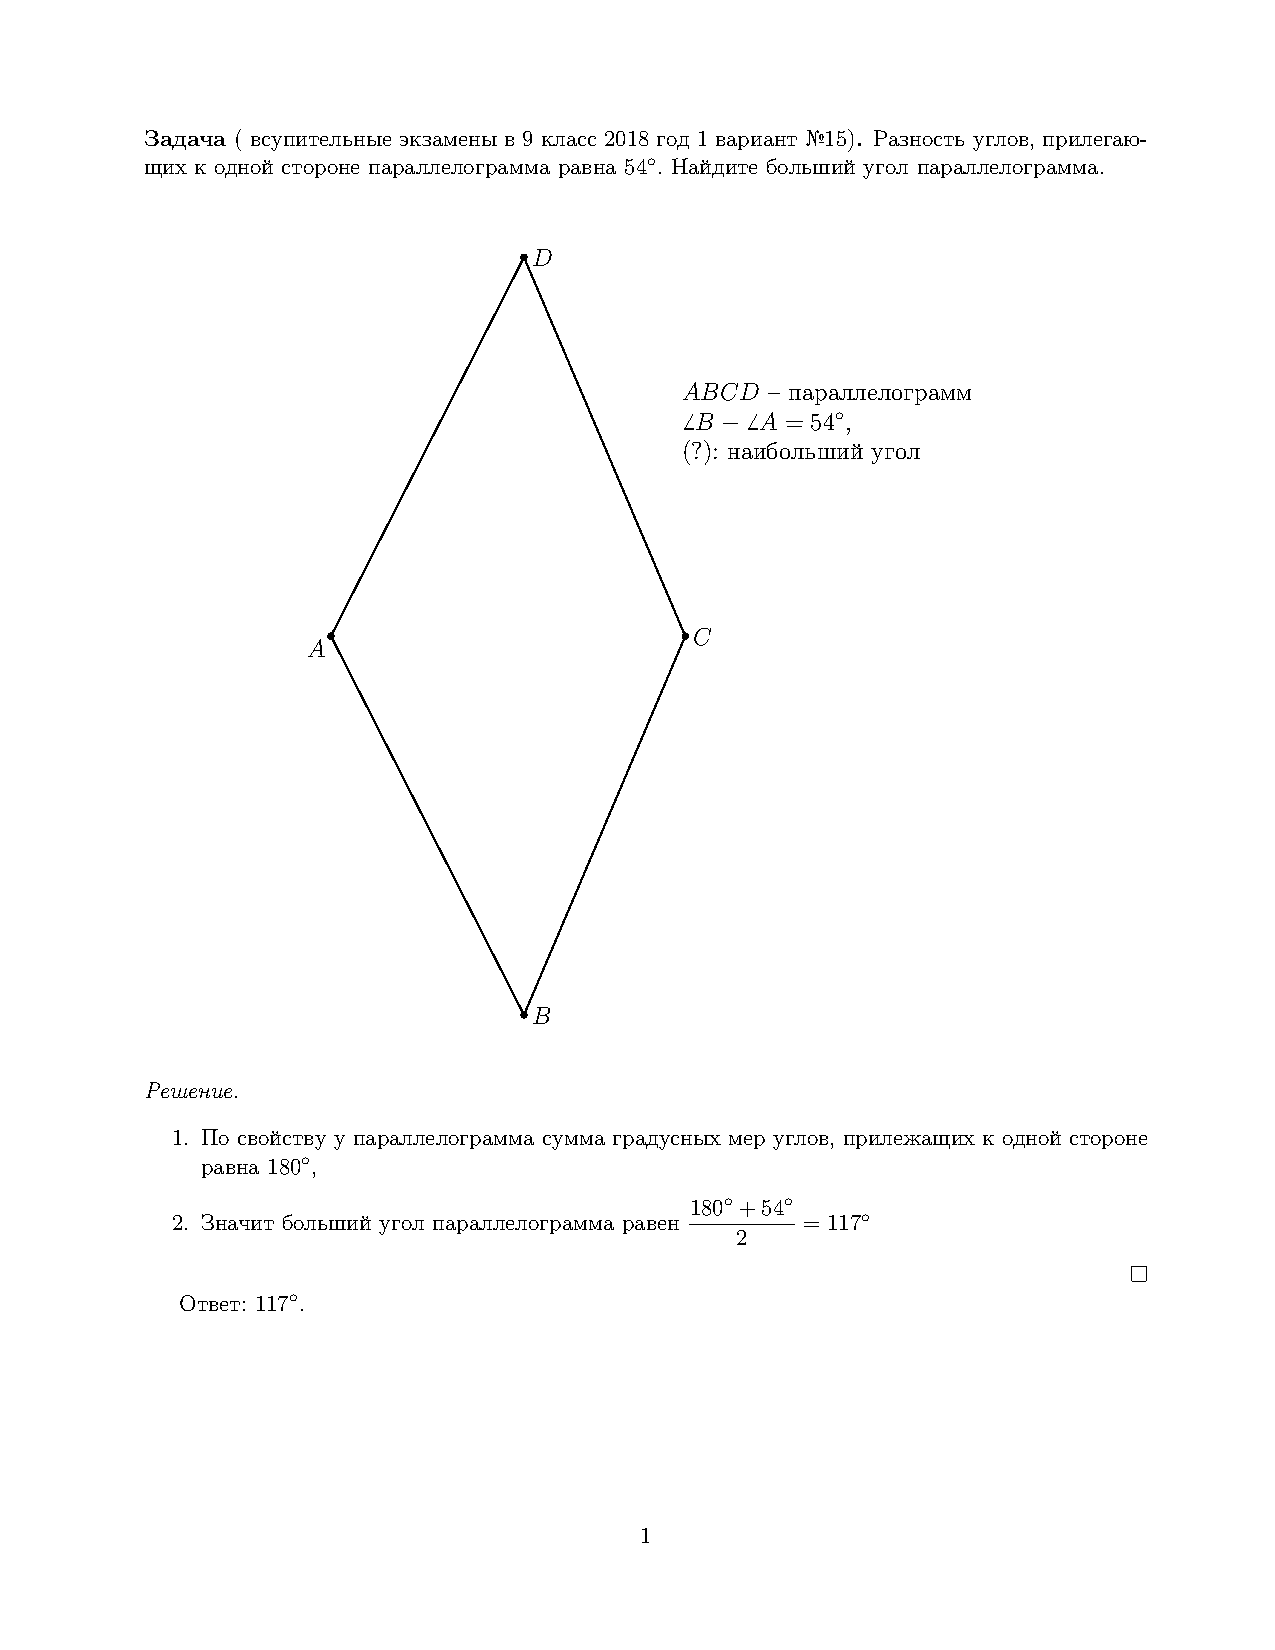
\includegraphics[scale = 1]{15.2.2018.pdf}}
	%\caption{ }\label{ris:task}
\end{figure}
\begin{proof}[Решение]\ 
\begin{enumerate}
\item  По свойству у параллелограмма сумма градусных мер углов, прилежащих к одной стороне равна $180^{\circ}$,

\item Значит больший угол параллелограмма равен $\dfrac{180^{\circ}+54^{\circ}}{2}=117^{\circ}$
\end{enumerate}
\end{proof}
\Answer{$117^{\circ}$}
\end{document}

